\section{Introduction}\label{sec:intro}

% P1: Motivation. 
% - What is the problem area you are working in and why is it important? 
% - Why is the problem of interest and importance to the larger community?
Recommender systems have become a hot research area in recent years and 
  many innovative approaches have been proposed both scientifically and commercially. 
Many recommender systems deal with books and daily commodities; 
  they need to be more efficient and accurate, and cover more fields.
Online trading is an overwhelming trend and E-commerce is a promising field. 
For many businesses, online opinion has turned into a kind of virtual currency 
  that can make or break a product in the marketplace. 
There are so many items (products) in E-commerce systems that 
  picking an item is time-consuming for individuals.
Therefore recommender systems are key to the success of such E-commerce systems, 
  and shortening the time for an individual means improving the 
  throughput of the E-commerce system, thus contributing more transactions.

% P2: What is the specific problem considered in this paper? 
The soaring E-commerce industry demands recommender systems 
  with higher efficiency and accuracy, as well as support for more 
  personalized recommendation.
Personalized recommendation can be achieved by using data mining techniques on 
  massive amount of user profiles and behaviors (so-called collaboration) 
  regardless of the features of recommended items themselves. 
However, this kind of personalized recommendation is not applicable to 
  personalized apparel recommendation where the choices of people with similar interests 
  are sensitive to apparel particulars and may differ in case of only tiny differences. 
In this case, it is essential to capture as many features as possible 
  which are associated with both the clothes themselves and the user's preference 
  so that the personalized recommendation can be achieved in better performance. 

% P3: Summarize what are the main contributions of your paper.
% - What is the general approach taken? 
% - Why are the specific results significant?
In this paper, we propose a novel idea and framework for personalized apparel recommendation
  which combines both item images and textual labels by using sparse coding and 
  support vector machine (SVM). 
Sparse coding provides a class of algorithms for finding succinct representations of stimuli; 
  given only unlabeled input data, it learns basis functions that capture higher-level features 
  in the data.
SVM is a widely used machine learning method for classification and regression analysis,
  based on the principle of structural risk minimization, which performs well when applied to 
  data outside the training set.

% P4: What are the differences in what you are doing, and what others have done?
% > In separate subsection `Related Work'
Given the images, the textual descriptions and the user ratings of the garments,
  our framework is capable of personalized recommendation according to various metrics
  such as style and diversity.
The novelty of our approach also comes from the fact that
  we try to not only employ a reasonable method to utilize 
  image information but also combine the image and text information together.
To the best of our knowledge, personalized apparel recommendation has not been 
  studied before in the context of E-commerce systems and the combination of 
  image feature extraction and machine learning.

\section{Overview}\label{sec:overview}

\begin{figure}
  \centering
  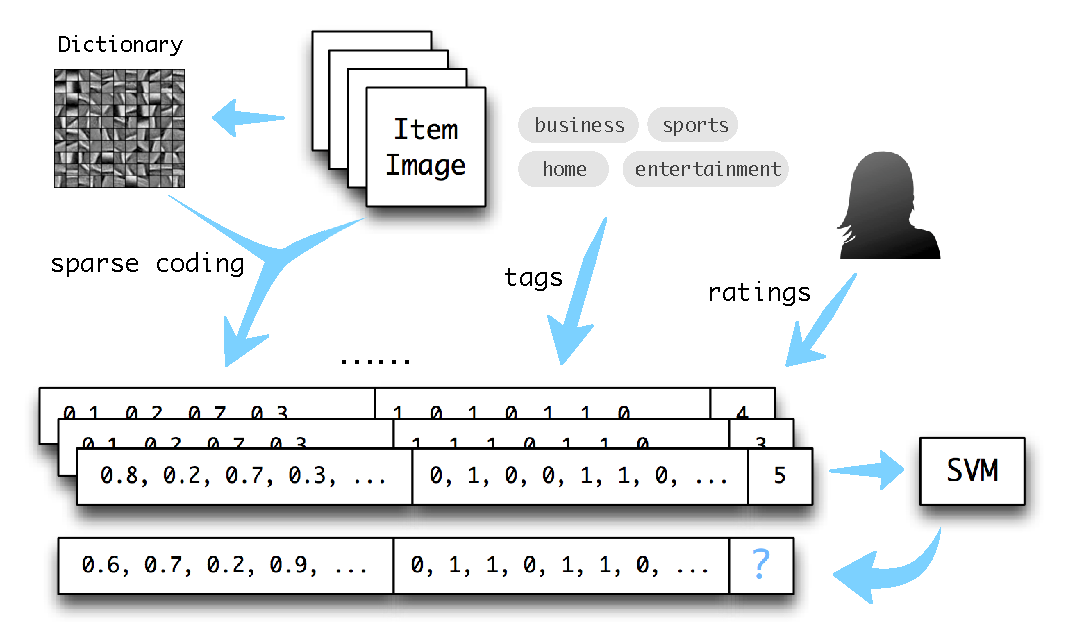
\includegraphics[width=0.9\textwidth]{framework}
  \caption{Framework Overview}
  \label{fig:framework}
\end{figure}

Our framework learned the features of clothing from both the textual labels and the images of clothes on the E-commerce websites. The input of our framework is the user preference which can be modeled from some of the user action records, including browsing time, favorite items, clicking history and ratings, etc. The output is the recommended clothes ranked by the possibility that the user would be interested in it. This framework has three major steps: learning clothing features,
modeling user preferences, and recommending by rating. Figure \ref{fig:framework} depicts the overall process of personalized recommendation in our framework.

\subsection{Learn clothing features}
There are two features we can leverage to model a garment item. One is textual labels such as cotton for material, sports for style and XL for size, etc. The other is several affiliated images depicting each garment. The information of textual labels and images would be represented as textual vectors and image vectors respectively. The representation of textual labels is quite straightforward as we can extract all the possible adjectives like slim, loose, lady and cute in the textual
labels. Each adjective represent a feature of the apparel in textual level. If the apparel item contains that feature in its textual label, we can mark 1 in the corresponding place of the textual vector. If not, mark 0. The image processing is more complicated than textual processing to learn the representations. We get the image vector from a base matrix which also serves as a dictionary. The technique details will be discussed in the paper. After both the textual labels
and the images being represented as vectors, the two vectors will be combined together by weight as the final representation for each apparel item.

\subsection{Model user preference}
In our framework, each apparel item is linked with a preference model for a specific user, and the model would be applied to map the clothing set to the preference set of that user. For different users, the mapping from the clothing set to the corresponding preference set may vary significantly. Many actions can be tracked in the E-commerce systems to model the user preference such as scanning time, favorite collection, purchase records and even clicks, etc. These features can be modeled
as a rating with an approriate range, 1 to 5 for instance. Here we choose the rating to represent the user preference is reasonable since the model of user preference has a direct connection with the way we do recommendation. If we model the user preference with ratings then we can recommend by the predicted ratings of each garment evaluated by machine learning technology. Quantify the user preference is an accurate and easy way to do the recommendation. 

\subsection{Recommend by rating}
The last step of our framework is to recommend clothes in which the user has high possibility to invest. The ranking strategy of the recommendation is based on the value of possibility provided by the machine learning technology which takes both the vectors of apparel item and the corresponding ratings of user preference as the input set. In this step, the major technique we've leveraged is support vector machine (SVM) which can solve this kind of problem correctly and efficiently. More details can been seen in the paper.\\
\\
In summary, there are three major contributions in this paper and our framework:
\begin{itemize}
	\item We propose a novel and more effective approach to build a framework for personalized apparel recommender systems which focus on the personality of different users and recommend with higher accuracy. We leverage all the possible information of each apparel item from both the textual labels and garment images. We combine the vectors of the two sources together by weight to represent the apparel item. The weight can be adaptive to different users as the emphasis on textual labels and images varied from person to person.
	\item We propose a novel way to leverage the different images affiliated to one apparel item. We treat these images as distinctive garment images with the same textual labels and ratings. For example, if an apparel item has ID 4 and contains 3 images I1 I2 I3 to dipict this garment along with a textual label T. If the corresponding preference of this garment has been known from a specific user and the rating is R. Then in our framework we treat these three images affiliated to the same
        apparel item as three distinctive items but with the same textual label T and the rating R. This process can enhance the efficiency of the item modeling and learning process.
	\item We have tried several algorithm that can be applied in our framework. As a consequence we managed to exclude the unsuitalbe ones and leverage the most efficient and suitable algorithms like HAC, K-SVD, SVM, etc.
\end{itemize}

